\documentclass[a4paper,11pt, twoside]{report}

\usepackage[czech]{babel}
\usepackage{fancyhdr}
\usepackage{tocloft}
\usepackage{footnote}
\usepackage{floatrow}
\usepackage{color}
\usepackage{geometry}
\usepackage{fontawesome}
\usepackage[useregional=numeric]{datetime2}
\usepackage{tikz}
\usepackage[pdftex,pdfhighlight=/P,colorlinks,linkcolor=blue]{hyperref}

\renewcommand\cftchapafterpnum{\vskip5pt}
\renewcommand\cftsecafterpnum{\vskip5pt}
\newfloatcommand{capbtabbox}{table}[][\FBwidth]
\geometry{a4paper, total={160mm,240mm}, left=25mm,  top=20mm, }

\usetikzlibrary{mindmap}
\usetikzlibrary{backgrounds}
    	
\pagestyle{empty}

\newcommand*{\info}[4][15]{%
  \node [ annotation, #3, scale=1.0, text width = #1em,
          inner sep = 2mm ] at (#2) {%
  \list{$\bullet$}{\topsep=0pt\itemsep=0pt\parsep=0pt
    \parskip=0pt\labelwidth=8pt\leftmargin=2pt
    \itemindent=0pt\labelsep=2pt}%
    #4
  \endlist
  };
}

\newcommand*{\infoX}[4]{%
  \node [ annotation, #3, scale=1.0, text width = #1em,
          inner sep = 4mm ] at (#2) {%
    #4
  };
}


\begin{document}


\pagestyle{myheadings}

\centering

\parbox{10mm}{
\vspace{70mm}
}

\pagestyle{empty}

{\Huge
\scalebox{2.5}{\faPencilSquareO}\\[2mm]
\textbf{Poznámky k psaní technických zpráv}\\[-0mm]
{
\normalsize
``středního'' rozsahu (např. k bakalářským/diplomovým pracím, projektové praxi),}\\[0mm]
{
\normalsize
k souvisejícím prezentacím, hodnocení aj.\\[4mm]
}
}
\scalebox{1.5}{
\normalsize
\textbf{v1.0}
}

\vspace{80mm}

\footnotesize
\flushright 
\parbox{2mm}{\vspace{1.5pt}\textsuperscript{\textcopyright}}~
\href{https://www.fit.vut.cz/person/strnadel/}{Josef Strnadel}, 
\href{https://www.fit.vut.cz/}{FIT VUT v Brně}.\\ 
Máte-li k dokumentu nějakou připomínku, dejte mi prosím vědět na \href{mailto:strnadel@fit.vut.cz}{strnadel@fit.vut.cz}.\\[+0mm]
Sazba pomocí \LaTeX{}, ikony z balíku \href{https://www.ctan.org/tex-archive/fonts/fontawesome}{fontawesome}.\\
Časové razítko dokumentu: \pdfcreationdate.  


\pagestyle{empty}

\pagebreak


\pagestyle{fancy}
\renewcommand{\headrulewidth}{0pt}
\renewcommand{\footrulewidth}{0pt}
\fancyhead{} 
\fancyfoot{} 
\fancyfoot[LE,LO]{\scriptsize \textit{Poznámky k psaní technických zpráv,  
\today
}}
\fancyfoot[CE,CO]{\scriptsize (\textit{\thepage})}  
\fancyfoot[RE,RO]{\scriptsize \parbox{2mm}{\vspace{1.5pt}\textsuperscript{\textcopyright}}~ \textit{\href{https://www.fit.vut.cz/person/strnadel/}{Josef Strnadel}, 
\href{https://www.fit.vut.cz/}{FIT VUT v Brně}}}

\newpage


\pagenumbering{roman}

\chapter*{Předmluva aneb ``pár slov na úvod''}


\vspace{-4mm}

\thispagestyle{fancy}



\flushleft



\faThumbsOUp~Hlavní \textbf{motivací pro vytvoření tohoto dokumentu} bylo shrnout odpovědi na, rok od roku se opakující podobné dotazy, 
které mi kladou ohledně \emph{technické zprávy} (\textsc{Tz}) ti, jejichž práce\footnote{bakalářské a diplomové práce, projektové praxe atp.} vedu na \href{https://www.fit.vut.cz/}{FIT VUT v Brně}. 


\quad




\faThumbsOUp~\textbf{Přínos pro studenty} očekávám ve
shrnutí srozumitelných a konzistentních odpovědí, které (snad a také snad snadno) v dokumentu naleznou; \textbf{přínosem pro mě} bude (snad) úspora času, který budu moci trávit více  odpovídáním pro zadání specifických než obecných, opakujících se dotazů. 


\section*{Co je účelem tohoto dokumentu?}

\begin{itemize}
\item[\faCheck]
\textbf{Posloužit} jako základní pomůcka při psaní \textsc{Tz}\footnote{primárně těm, jejichž práce vedu na \href{https://www.fit.vut.cz/}{FIT VUT v Brně}; 
ostatní mohou text využít také, ale pohled jejich vedoucího, zvyklosti jejich instituce atd. se od těch mých mohou lišit}, jako ``minigalerie'' možností \LaTeX, stylů psaní atp.,
\item[\faCheck] 
\textbf{objastnit} nejčastější pochybnosti ohledně struktury a obsahu\footnote{tj. textu, doprovodných ilustrací atd.} \textsc{Tz},
\item[\faCheck] 
\textbf{inspirovat}\footnote{spíše přehledově-ilustrativním než vyčerpávajícím způsobem} ke kvalitní struktuře a obsahu \textsc{Tz} 
a~\textbf{povzbudit} k prohlédnutí odevzdaných \textsc{Tz} a jejich hodnocení u~proběhnutých SZZ\footnote{viz např. \url{www.fit.vut.cz/study/theses/}} 
či obdobných rad\footnote{viz např. \url{www.herout.net/tao-diplomky/}},
\item[\faClose] 
\textbf{rozhodně NE} nahradit pokyny k pracím a SZZ\footnote{viz \url{www.fit.vut.cz/study/theses/bachelor-theses/},
\url{www.fit.vut.cz/study/theses/master-theses/} aj.}, 
opakovat všeobecně známé typografické či jiné zásady,
dávat lekce z \LaTeX u,
nutit konkrétní strukturu/obsah \textsc{Tz},
omezovat Váš projev,
nahrazovat či upravovat pokyny od vedoucího Vaší práce
apod.
\end{itemize}

\quad

\tikzstyle{background rectangle}=[thin,draw=black]

\label{ref:research}

\begin{savenotes}
\begin{tikzpicture}[show background rectangle, rounded corners=5pt]

\node[align=justify, text width=0.95\textwidth, inner sep=.5em]{
\textbf{Prokažte} své \textbf{studijní\footnote{slovo ``student'' je odvozeno z latinského ``studeo, studere'', tj. ``snažit se'', předpokládajícího aktivitu}
schopnosti} --
\textbf{hledejte}/\textbf{zpracovávejte}\footnote{zejména během počáteční rešeršní etapy; více viz např. část \ref{sec:research}, str. \pageref{sec:research}} relevantní \textbf{informace} 
k zadanému tématu
a
\textbf{klaďte}\footnote{ať už sami sobě či někomu ze svého okolí; bez otázek se hledá těžko a bez hledání většinou nic nenajdete}
\textbf{otázky} 
(nejen) k \textsc{Tz}\footnote{začněte např. pročtením těchto zdrojů: 
\href{https://www.theiet.org/media/5182/technical-report-writing.pdf}{TheIET},
\href{https://ias.ieee.org/images/files/CMD/2020/2020-01-16_IET_Technical_Report_Writing_Guidelines.pdf}{IEEE},
\href{https://students.unimelb.edu.au/academic-skills/resources/report-writing/technical-report-writing}{UniMELB},
\href{https://www.sussex.ac.uk/ei/internal/forstudents/engineeringdesign/studyguides/techreportwriting}{US}}. 
%
Při \textbf{hledání} 
\textbf{VŽDY čerpejte z více nezávislých, důvěryhodných zdrojů}, informace nepřebírejte bezhlavě, ale
\textbf{obezřetně}\footnote{i mistr tesař se někdy 
``utne'' -- může např. šířit neověřené (vágní, povrchní, zavádějící aj.) informace}.
\textbf{Snažte se} odvést práci, jejíž výsledek bude nejen kvalitní, ale i něčím kladným zaujme (např. nekonvenčním přístupem, vlastnostmi, aplikačním potenciálem, společenskou prospěšností či ohlasem od uživatelů).
};

\node[xshift=3ex, yshift=0ex, overlay, fill=white, draw=white, above 
right] at (current bounding box.north west) {
\parbox{3mm}{\rotatebox{0}{\scalebox{1.5}{\faThumbTack}}\vspace{-2mm}}
};

\end{tikzpicture} 
\end{savenotes}


\section*{Jak se orientovat v následujícím textu?}

Kap. 
\ref{chapt:tech-rep-notes}
(str. \pageref{chapt:tech-rep-notes})
shrnuje rady, kterých se vhodné se držet a nedostatků, kterých je vhodné se vyvarovat při psaní \textsc{Tz},
kap.
\ref{chapt:tech-rep-struct}
(str. \pageref{chapt:tech-rep-struct})
se snaží inspirovat k vytvoření kvalitní struktury \textsc{Tz},
příloha
\ref{chapt:eval}
(str. \pageref{chapt:eval})
se zabývá 
hodnocením přípravy na řešení daného tématu
a příloha
\ref{chapt:prez}
(str. \pageref{chapt:prez})
shrnuje rady pro tvorbu prezentace a její přednes publiku.
	

\vspace{4mm}
\flushright

\includegraphics[scale=.35]{my_signature}


\emph{Josef Strnadel, autor}


\vspace{2mm}


\raggedbottom

\pagebreak

\flushleft



\tableofcontents


\thispagestyle{empty}


\raggedbottom

\thispagestyle{fancy}


\pagebreak

\pagenumbering{arabic}


\chapter{Než začnete psát \textsc{Tz} \ldots}
\label{chapt:tech-rep-notes}


\thispagestyle{fancy}

\vspace{-4mm} 

Pokud máte 
vedoucího a téma práce, které 
máte rozpracováno do té míry, že již uvažujete o psaní \textsc{Tz},
následující text je právě pro Vás; potřebujete-li poradit s volbou tématu, získat představu o průběhu řešení apod., 
 můžete se informovat např. na 
\url{www.herout.net/tao-diplomky/}.

\quad 

\quad 

\parbox{\textwidth}{
\centering 

\scalebox{2.5}{

\faCheck
}}

\section*{Několik ``užitečných'' rad}

\begin{itemize}
\item[\faCheck]
Pokud to nic nevylučuje, 
\textbf{pište v jazyce, ve kterém nemáte problém vyjádřit své myšlenky}\footnote{dostanete-li se, např. kvůli problémům při řešení, do časové tísně, jazyk může sehrát klíčovou roli, 
ať už z~hlediska dodržení termínu odevzdání či čitelnosti \textsc{Tz}}; 
pro globálnější dopad/ohlas je lepší psát \textsc{Tz} v angličtině a její výsledky zviditelnit
(\href{https://github.com/}{\faGithub}, \href{https://www.vut.cz/vut}{soutěže} aj.),

\item[\faCheck]
\textbf{buďte jednotní} v jazyce hlavního textu a ilustrací, ve stylu definic a informací uváděných výčtem aj.,

\item[\faCheck]
\textbf{používejte kontrolu pravopisu}\footnote{angl. spell-checker}
-- dokáže odhalit mnohé chyby a~není tedy rozumný důvod, proč ji nevyužít;
odhalit a opravit gramatické či významové nedostatky je již mnohem obtížnější -- ideální je dát text někomu přečíst; 
v případě pochybností doporučuji také nahlédnout např. do (této či jiné) \href{https://prirucka.ujc.cas.cz/}{příručky},

\item[\faCheck] 
(správně) \textbf{používejte obvyklé}\footnote{v dané oblasti zájmu zavedené} pojmy atp.; 
případné \textbf{zkratky/symboly} atp. \textbf{definujte} předtím, než je použijete -- např. význam některých 
zkratek\footnote{např. RTL: Real-Time Logic $\times$ Register-Transfer Level} 
se může v různých oblastech lišit, což může čtenáře zmást,

\item[\faCheck] 
nejedná-li se o všeobecně známá fakta, tak jasně \textbf{identifikujte aktéry} a \textbf{autory}, 
např. namísto 
``mnohé práce prokázaly'', ``bylo vytvořeno'', ``činnost A je prováděna'' apod.
uvádějte raději 
``autoři publikací \dots ~zjistili'', ``vytvořil jsem'', ``činnost A provádí algoritmus/procesor B'',

\item[\faCheck]
``větší množství''\footnote{subjektivně cca 2 strany, záleží ale např. i na kontextu a ``hutnosti'' předkládané informace} souvislého textu doplňte o \textbf{ilustraci}; 
nepotřebujete-li nutně mnohabarevnou bitmapovou ilustraci\footnote{např. fotografii reality}, 
použijte\footnote{typicky pro diagramy, schémata, tabulky atp.} raději \textbf{kontrastní}, ideálně \textbf{vektorovou} ilustraci;
u~\textbf{grafů} dbejte na \textbf{popisky os}, 
u~\textbf{fyzikálních veličin} nejen na jejich hodnotu, ale také na jejich (správnou a správně formátovanou)\footnote{např. ``Obvodem tekl proud $5~mA$ (pět miliampér).'' $\times$ ``Obvodem tekl $5mA$ (pětimiliampérový) proud.''} 
jednotku atp.,


\item[\faCheck] při odkazování se na objekty \textbf{nezapomínejte uvádět typ odkazovaného objektu}\footnote{``více informací najdete v \ref{sec:C-1},
\ref{fig:C-1},
\ref{tbl:C-1}''
$\times$
``více informací najdete v~odst. \ref{sec:C-1},
obr. \ref{fig:C-1},
tab. \ref{tbl:C-1}''}; 
\textbf{správnost odkazů}
a \textbf{funkčnost} hypertextových \textbf{odkazů ověřte}.


\end{itemize}

\pagebreak


\raggedbottom


\parbox{\textwidth}{
\centering 

\scalebox{2.5}{

\faClose
}}


\section*{Výběr z toho, čemu se vyhnout}


\raggedbottom


\begin{itemize}
\item[\faClose] 
\textbf{Opakování}\footnote{připomenutí dříve sděleného může být užitečné, 
nicméně ne tak opakování stejných, delších úseků textu} 
dříve sdělené informace,
nedostatků (např. překlepy, špatná práce s hodnotami a~jednotkami fyzikálních veličin, vícenásobná definice zkratek a symbolů, ``bílé místo''\footnote{srov. např. rozmístění obr. \ref{fig:C-1}, tab. \ref{tbl:C-1} $\times$ obr. \ref{fig:C-2}, tab. \ref{tbl:C-2}} v textu, 
přesah textu přes okraj stránky) apod., 

\item[\faClose] 
\textbf{nesprávným}, \textbf{neobvyklým}\footnote{např. neznalost zavedeného názvosloví budí ve čtenáři pochybnosti o tom, zda se v dané oblasti orientujete}
 či jinak \textbf{nevhodným} výrazům, např. 
``nejoptimálnější'' či 
``nejideálnější'',
``komplexita'',
``fíčura''\footnote{z angl. ``feature'', česky ``vlastnost'', ``rys''},
``pík''\footnote{z angl. ``peak'', česky ``vrchol'' },
\item[\faClose]  
\textbf{vágním}, \textbf{povrchním}, \textbf{zavádějícím} atp. informacím, např.
``vykoná se okamžitě\footnote{okamžitě znamená ``v témže čase''; vykonání práce při neplynutí času však vyžaduje nekonečný výkon}'',
``teplota je řádově\footnote{upřesněte -- řády jsou, např., desetiny, jednotky, desítky, stovky, \ldots} ve stupních Celsia'',
``spotřeba energie je vysoká'',
``frekvenční rozsah je široký'', 
``citelně vyšší výkon'',



\item[\faClose] 
\textbf{tvrzením},  zejména pak \textbf{závěrům} \textbf{nepodloženým\footnote{předem či v rámci příslušného sdělení} daty}, 
např. 
``využil jsem části převzatých programů'',
``zdá se mi, že vše funguje, jak má'' či ``realizované zařízení pracuje normálně a~bezchybně'',
``náš přístup předčí dříve publikované přístupy'',
``předložené řešení je škálovatelné a~univerzálně použitelné'',

\item[\faClose] 
\textbf{nejasnostem} a
\textbf{nezodpovězeným otázkám}
ohledně realizovaného díla
-- v \textsc{Tz} 
představte zejména:
\begin{itemize}
\item
požadovaný \textbf{účel} díla, jeho očekávaný \textbf{přínos}
a
stěžejní \textbf{požadavky} kladené na dílo,
\item
existující \textbf{přístupy} k realizaci obdobných děl a jejich \textbf{ne/výhody},
\item
\textbf{metody}, \textbf{prostředky}, \textbf{technologie} a \textbf{prvky} použitelné/použité při realizaci díla, jejich \textbf{vlastnosti}/\textbf{provázanost}, 
\item
\textbf{mechanismus činnosti} díla a 
\textbf{způsob užití} díla,
\item
\textbf{způsob/prostředky} \textbf{zhodnocení} díla a~\textbf{vlastnosti} díla; 
\end{itemize}
u možných alternativ zdůvodněte \textbf{rozhodnutí pro} konkrétní \textbf{volbu}.

\end{itemize}

\vspace{20mm}

\parbox{\linewidth}{
\centering

\scalebox{10.0}{
\faBug
}
}

\vspace{20mm}

\pagebreak

\chapter{Orientační struktura \textsc{Tz}}
\thispagestyle{fancy}

\raggedbottom

\label{chapt:tech-rep-struct}

\vspace{-6mm}

Než se pustíte do rozsáhlejšího psaní, 
doporučuji \textbf{rozvrhnout si strukturu} \textsc{Tz} a~\textbf{prodiskutovat ji} se svým vedoucím.\footnote{projděte si např. technické zprávy a jejich hodnocení na \url{www.fit.vut.cz/study/theses/},
rady na \url{www.herout.net/blog/2012/03/struktura-diplomove-prace/} či 
\url{https://www.herout.net/blog/2013/04/jak-pojmenovat-kapitoly-v-odbornem-textu/}
}
Níže jsem se pokusil o výtah toho, co by v žádné \textsc{Tz} nemělo chybět. 
Některé \textbf{názvy} (pod)kapitol apod. mohou být \textbf{dány} např. konkrétními \textbf{předpisy},
jiné názvy si naopak \textbf{autor může  upravit/zvolit}\footnote{v takovém případě volte název tak, aby stručně a srozumitelně, přitom však co nejlépe, vystihoval stěžejní informace, o nichž příslušná část textu pojednává}.


\section{Abstrakt}

\vspace{-1mm}

\ldots 
~\textbf{stručně shrnuje}
 informace shromážděné v rozsáhlejším dokumentu (v~našem případě \textsc{Tz}) s cílem \textbf{zaujmout} 
a \textbf{usnadnit} tak případnému zájemci o čtení dokumentu \textbf{rozhodnout} se,
zda je přínosné věnovat čtení dokumentu čas. 
%
Abstrakt\footnote{více viz např. \href{https://www.herout.net/blog/2013/12/jak-psat-abstrakt/}{herout.net/blog}}, mj.,  
\textbf{přehledově představuje} problém,
popisem jehož řešení se dokument zabývá, 
(očekávaný) cíl a přínos vlastního řešení,
stěžejní metody, prostředky a vlastní přístup k~jeho řešení,
zdůrazňuje stěžejní dosažené výsledky a zjištěné závěry
a porovnává je s dosavadními/publikovanými.

\vspace{3mm}


\begin{savenotes}
\begin{tikzpicture}[show background rectangle, rounded corners=5pt]

\node[align=justify, text width=0.75\textwidth, inner sep=.5em]{
\dots
~je \textbf{typicky poměrně krátký}, tj. obsahuje cca 200 -- 400 slov.};

\node[xshift=3ex, yshift=0ex, overlay, fill=white, draw=white, above 
right] at (current bounding box.north west) {
\parbox{3mm}{\rotatebox{0}{\scalebox{1.5}{\faThumbTack}}\vspace{-2mm}}
};

\end{tikzpicture} 
\end{savenotes}

\vspace{-1mm}

\section{Klíčová slova}


\dots
~\textbf{heslovitě charakterizují} zásadní sdělení dokumentu
a 
\textbf{identifikují} stěžejní oblasti, problematiku a~téma(ta),
kterými se dokument zabývá, jakož i klíčové metody, prostředky a technologie použité při realizaci dokumentovaného díla. 
%
Klíčová slova\footnote{více viz např. 
\href{https://kisk.phil.muni.cz/media/3089574/kisk.phil.muni.cz/kpi/temata/definovani-tematu/klicova-slova.html}{phil.muni.cz}
či \href{http://iva.k.utb.cz/lekce/co-jsou-klicova-slova-a-jak-je-tvorit/}{IVA}.
} 
\textbf{jsou 
zpravidla jedno/víceslovné výrazy} představující známá\footnote{všeobecně či v oblasti zadaného tématu} slovní spojení, jména, názvy, místa, události atp.; nejedná-li se o jméno, název či zkratku, začínají malým písmenem.

\tikzstyle{background rectangle}=[thin,draw=black]

\vspace{4mm}

\begin{savenotes}
\begin{tikzpicture}[show background rectangle, rounded corners=5pt]

\node[align=justify, text width=0.960\textwidth, inner sep=.5em]{
\vspace{-2mm}

\textbf{Př. 1} (\textbf{téma} ``Digitální zvuková steganografie''); 
\textbf{klíčová slova:}
bezpečnost, ukrývání informací, digitální steganografie, zvuk, PCM, WAV, Fourierova transformace, Python, nejméně významný bit, ozvěna, rozprostřené spektrum, fázové kódování, paritní kódování, vkládání tónu, úseky ticha, vlnková transformace

\vspace{2mm}

\textbf{Př. 2} (\textbf{téma} ``Rozšíření řídicího systému modelu letadla Skydog o podporu vzdáleného a samočinného řízení Android aplikací''); 
\textbf{klíčová slova:}
autopilot, APM, Arduino, Android, bezpilotní letadlo, UAV, UAS, MAVLink, DTM, RRT, GeoTIFF, protisrážkový systém

\vspace{2mm}

\textbf{Př. 3} (\textbf{téma} ``Bezdrátový hlasovací systém založený na IEEE 802.15.4/Zigbee''); 
\textbf{klíčová slova:}
IEEE 802.15.4, ZigBee, bezdrátové hlasování, Freescale 1321xNSK, Java, RXTX, XML, JDOM, PHP



\vspace{2mm}

\textbf{Př. 4} (\textbf{téma} ``Výpočetní model a analýza energeticky úsporných budov''); 
\textbf{klíčová slova:}
budova, parametry, prostředí, materiál, topení, chlazení, profil uživatele, chování, spotřeba energie, řízení, energetická úspora, optimalizace, modelování, simulace, verifikace, časované automaty, modální logika, UPPAAL


};

\node[xshift=3ex, yshift=0ex, overlay, fill=white, draw=white, above 
right] at (current bounding box.north west) {
\parbox{3mm}{\rotatebox{0}{\scalebox{1.5}{\faThumbTack}}\vspace{-2mm}}
};

\end{tikzpicture} 
\end{savenotes}



\pagebreak

\parbox{\textwidth}{
\centering

\scalebox{2.5}{
\faSupport
}
\vspace{-8mm}
}

\section{Úvod}

\ldots 
~\textbf{bývá} zpravidla \textbf{krátký}, o rozsahu cca 1--2 stran.
Pokud se čtenář pustil do jeho čtení, tak jej \textsc{Tz} již něčím zaujala 
a úvod by měl posílit jeho touhu číst dále.
V úvodu především 
stručně (a jinými slovy než v abstraktu) 
\textbf{shrňte důvod/motivaci} zabývat se řešením zadaného tématu
a
\textbf{očekávaný cíl a přínos} vlastního přístupu k~řešení.
Zakončit jej můžete stručným komentářem struktury \textsc{Tz}.

\parbox{\textwidth}{
\centering

\scalebox{2.5}{
\faBook
}
\vspace{-8mm}
}

\section{Rešerše}
\label{sec:research}

Řešením zadaného tématu 
byste se měli vážněji zabývat 
až po \textbf{předchozí} důkladné a co nejširší \textbf{rešerši} relevantních informací 
souvisejících s tématem -- \textbf{VŽDY čerpejte z více nezávislých, důvěryhodných zdrojů}. 
Informace \textbf{nepřebírejte bezhlavě},
\textbf{nepracujte s 
neověřenými} (vágními, povrchními, zavádějícími aj.) \textbf{informacemi}.


\subsection{Zadané téma a související problematika}

Nashromážděné informace nejprve \textbf{uspořádejte}, vč. zažité terminologie atp.,
a s jejich využitím 
\textbf{uveďte čtenáře}, srozumitelně a nesporně, \textbf{do oblasti} řešeného tématu
a \textbf{jasně formulujte řešený problém}.
\textbf{Shromažďujte} stěžejní informační zdroje.

\subsection{Existující přístupy k řešení}


Poté, co nejšířeji,
\textbf{shrňte, klasifikujte a charakterizujte} (stěžejní, ale i okrajové) 
prostředky, metody a~přístupy používané k~řešení daného problému
vč. 
jejich ne/výhod.
\textbf{Shromažďujte} informační zdroje ke~stěžejním (reprezentativním) přístupům.

\vspace{8mm}

\parbox{\textwidth}{
\centering

\scalebox{2.5}{
\faCogs
}
\vspace{-4mm}
}


\section{Rozbor realizačních možností a návrh řešení}

Následně \textbf{shrňte}\footnote{jasně, stručně, ale, pokud možno, co nejvíce konkrétně (požadavky kladené  na výsledné řešení, podmínky a~případy jeho užití atp.)}, \textbf{co plánujete vytvořit}, \textbf{čím chcete přispět} k řešení daného problému a \textbf{jak} 
tento očekávaný příspěvek \textbf{plánujete ověřit}. \textbf{Proveďte rozbor} realizačních možností, tj. 
zvažovaných prostředků, technologií, metod a~přístupů k řešení a na jeho základě \textbf{zvolte}\footnote{volbu dostatečně a srozumitelně odůvodněte} ty, které 
se jeví jako nejvíce vhodné. \textbf{Představte stěžejní činnosti} nezbytné k dokončení řešení,
jejich \textbf{návaznosti} a~\textbf{harmonogram}.

\vspace{8mm}

\parbox{\textwidth}{
\centering

\scalebox{2.5}{
\faPencil
}
\vspace{-8mm}
}



\section{Popis řešení}

Konkrétně a srozumitelně \textbf{popište} vše stěžejní, \textbf{co} (prostředky\footnote{hardware (platformy, komponenty atp.), software (dostupné nástroje, knihovny atp.), datové sady aj.}) \textbf{a jak} (metody, přístup) \textbf{jste využili}, \textbf{které činnosti jste vykonali} při řešení zadaného tématu, \textbf{s jakými obtížemi} jste se při řešení \textbf{potýkali}, co bylo jejich příčinou, jak byly závažné a jak jste se s nimi vypořádali.
\textbf{Přesvědčte čtenáře}, že jste vykonali nezanedbatelné množství práce, jejímž výsledkem je dílo, které nejenže splňuje požadavky zadání, ale které je (ideálně) také kvalitní. 
Pokud \textbf{dílo zcela nesplňuje požadavky zadání}, 
zdůrazněte a zdůvodněte to.
\textbf{Nezahlťte čtenáře} nadměrným množstvím informací -- případné informace doplňkového charakteru\footnote{výtahy z technické dokumentace, úplná/rozsáhlejší schémata, algoritmy či programy atp.} odsuňte \footnote{ideálně po předchozí konzultaci s vedoucím} 
raději
do příloh.
\textbf{Nedopusťte, aby} po dokončení četby \textbf{zbyla čtenáři řada nezodpovězených otázek} zejména ohledně jádra/těžiště řešení daného tématu.


\pagebreak

\vspace{8mm}

\parbox{\textwidth}{
\centering

\scalebox{2.5}{
\faAreaChart
}
\vspace{-8mm}
}


\section{Zhodnocení řešení}

Konkrétně a srozumitelně \textbf{popište, pomocí čeho} (prostředky, technologie) \textbf{a jak} (metody) \textbf{jste zjišťovali}, že vytvořené dílo splňuje požadavky na něj kladené zadáním -- zjištěný \textbf{závěr podložte daty}\footnote{vhodně zpracované výsledky experimentů, uživatelského testování, dotazníkového šetření atp.};  
\textbf{nezahlťte čtenáře} nadměrným množstvím informací -- případné informace doplňkového charakteru\footnote{detailní nezpracovaná/hrubá data, hledání příčin nedostatků atp.} odsuňte\footnote{ideálně až po předchozí konzultaci s vedoucím} raději do příloh.
Při hodnocení díla 
\textbf{nezastírejte realitu} a
\textbf{buďte kritičtí} -- zhodnoťte, za jakých okolností jsou data příznivá a za jakých nepříznivá; v druhém případě analyzujte příčinu\footnote{pokud se něco nepovedlo, nefunguje, jak má apod., pokuste se odhalit příčinu a vše zdokumentujte} a dopad na splnění požadavků zadání. 
\textbf{Nedopusťte, aby} po dokončení četby \textbf{nabyl čtenář pochybnosti} ohledně splnění požadavků zadání.




\vspace{8mm}

\parbox{\textwidth}{
\centering

\scalebox{2.5}{
\faLegal
}
\vspace{-8mm}
}



\section{Závěr}

Závěr, obdobně jako úvod, \textbf{bývá} zpravidla \textbf{krátký}, o rozsahu cca 1--2 stran.
Někteří čtenáři se však rozhodnou číst hlavní text \textsc{Tz} až poté,
co usoudí mj.\footnote{tedy nejen z názvu, klíčových slov, abstraktu} ze závěru, že \textsc{Tz} by pro ně mohla být přínosná.
Na~závěru \textsc{Tz} si tedy dejte záležet\footnote{přesvědčte potencionálního čtenáře, že má smysl věnovat čtení \textsc{Tz} čas}, aby více přitahoval než odpuzoval potencionální čtenáře  -- především v něm
stručně 
\textbf{připomeňte důvod/motivaci} zabývat se řešením zadaného tématu,
očekávaný cíl a přínos vlastního přístupu k řešení;
\textbf{charakterizujte vlastní přístup k řešení} a~při něm použité (stěžejní) prostředky, technologie a~metody;
\textbf{shrňte přístup ke zhodnocení řešení}\footnote{podmínky/scénáře, datové sady, prostředky a metody sběru, zpracování a vizualizace dat, jejich rozsah atp.},
stěžejní dosažené výsledky a zjištěné závěry,
co indikují\footnote{``Co se ne/povedlo?'', jaké má řešené vlastnosti na jaké třídě aplikací, za jakých podmínek atp.}
a~jejich srovnání s dosavadními/publikovanými.

\vspace{8mm}

\parbox{\textwidth}{
\centering

\scalebox{2.5}{
\faList
}
\vspace{-8mm}
}



\section{Seznam citací}

Tento seznam\footnote{typicky o cca 20-40 položkách} by měl obsahovat \textbf{stěžejní informační zdroje}
k rešerši i řešení zadaného tématu. 
Na zdroje z~tohoto seznamu by se \textsc{Tz} měla \textbf{odkazovat}\footnote{ideálně s rovnoměrným rozložením}, 
aby
\textbf{zdůraznila} aktuálnost řešené problematiky
a potřebu zabývat se jí,
\textbf{shrnula} dosavadní přístupy, prostředky a metody k jejímu řešení a zhodnocení jejich vlastností, 
\textbf{podpořila} příslušná tvrzení a úsudky,
\textbf{jasně odlišila} prvky existující/převzaté využité při realizaci od prvků vlastních atp.
Zdroje by měly být důvěryhodné, ideálně recenzované, a nesporně identifikovatelné.

\vspace{8mm}

\parbox{\textwidth}{
\centering

\scalebox{2.5}{
\faTags
}
\vspace{-8mm}
}




\section{Přílohy}


\thispagestyle{fancy}

Do příloh můžete vložit případné \textbf{informace}\footnote{smysluplné a k tématu relevantní} \textbf{doplňkového charakteru}, např. výtahy z technické dokumentace; úplná, rozsáhlejší či detailnější schémata, algoritmy či programy, nezpracovaná a hrubá data; hledání příčin nedostatků a 
návod na zprovoznění vytvořeného díla; uživatelskou příručku k vytvořenému dílu; uspořádání a strukturu informací uložených na paměťovém médiu přiloženému k \textsc{Tz} atp.



\pagebreak



\appendix

\thispagestyle{fancy}


\chapter{Hodnocení přípravné etapy}

\label{chapt:eval}

\raggedbottom

\vspace{-8mm}

\ldots
probíhá \textbf{cca v polovině doby} vyhrazené pro řešení projektu, 
tj. zpravidla po skončení prvního semestru vyhrazeného pro řešení.
Pro co \textbf{nejobjektivnější hodnocení} používám následující \textbf{pomůcku}
(obr. \ref{fig:eval}, tab.~\ref{tbl:eval}) 
-- můžete ji využít  k~(alespoň hrubému/orientačnímu) \textbf{odhadu hodnocení}.

\thispagestyle{fancy}

\vspace{-0mm}
\begin{figure}[h]
\rotatebox{0}{
\scalebox{.3}{
\hspace{-250mm}
\begin{tikzpicture}[ every annotation/.style = {draw, 
                     fill = none, 
                     font = \huge},
    mindmap,
    grow cyclic, text width=2.5cm, align=flush center, 
    every node/.style={concept, 
    font = \Large},
    concept color=black, 
root concept/.append style={concept color=black, line width=2ex, fill=white, text=black, font=\large\scshape},
    level 1/.style={level distance=8cm,sibling angle=100, text width=45mm},
    level 2/.style={level distance=6.5cm,sibling angle=45, text width=40mm}]

\node (total) [root concept, text width=6.0cm] {\Huge \bf $\sum$\\[2mm]Celkové hodnocení\\[4mm] (100)}
    child [concept color=green!100!red!50] { node (activity) {\bf \huge E\\Přístup\\(10)}
    }
    child [concept color=yellow!75] { node (progress) {\bf \huge R\\Rozpraco-- vanost\\[2mm](30)}
        child [concept color=yellow!25] { node(eval_proposal) {\huge Návrh\\[-1mm]zhodnocení\\[-1mm]řešení\\(10)}}
        child [concept color=yellow!25] { node(readiness) {\huge Připravenost\\[-1mm]k~řešení\\(10)}}
        child [concept color=yellow!25]{ node(preliminary_results) {\huge Průběžné\\[-1mm]výstupy\\(10)}}
    }
    child [concept color=blue!25] { node (pres) {\bf \huge P\\Prezentace\\[2mm](30)}
        child [concept color=blue!10] { node(defense) {\huge Obhajoba\\(10)}}
        child [concept color=blue!10]{ node(clarity) {\huge Srozumitelnost\\[2mm](10)}}
        child [concept color=blue!10]{ node(timing) {\huge Načasování\\(10)}}
    }
    child [concept color=gray!50] { node (doc) {\bf \huge T\\[2mm]Technická zpráva\\[2mm] (30)}
        child [concept color=gray!25]{ node(text) {\huge Čitelnost\\(10)}}
        child [concept color=gray!25]{ node(analysis) {\huge Rešerše\\[-1mm]a rozbor\\[0mm](10)}}
        child [concept color=gray!25]{ node(proposal) {\huge Návrh\\[-1mm]řešení \\(10)}}
    };
%
\infoX{30}{text}{above,anchor=east,xshift={5em}, yshift=7em,concept color=black}{
        Strukturování, jazyková, typografická a~odborná úroveň a srozumitelnost textu, ilustrativnost, ...}
\infoX{14}{eval_proposal.west}{above,anchor=east,xshift={2em}, yshift=0em,concept color=black}{
        Jasnost a reálnost představy o~zhodnocení řešení,~...}
\infoX{25}{defense.south}{above,anchor=north,xshift=10em, yshift=2em,concept color=black}{
        Schopnost reagovat na dotazy, obhájit svá tvrzení, ...}
\infoX{30}{clarity}{above,anchor=south,xshift=15em, yshift=3em,concept color=black}{
        Srozumitelnost sdělení, jasnost myšlenkové linie a držení se jí, úprava snímků, vhodnost ilustrací, ...}
\infoX{15}{timing.west}{above,anchor=east,xshift=1em, yshift=0em,concept color=black}{
        Vhodnost rozložení toku informací v~čase, dodržení časového limitu, ...
        }
\infoX{25}{activity.west}{above,anchor=east,xshift=2em, yshift=0em,concept color=black}{
 Včasnost zahájení prací, snaha o~netriviální a kvalitní řešení, průběžnost práce, konzultace řešení, ...
 }
\infoX{35}{analysis.west}{above,anchor=east,xshift=2em, yshift=0em,concept color=black}{
 Představení oblasti k tématu, shrnutí terminologie atp.;
 definice a rozbor řešeného problému, kritické shrnutí  přístupů k~řešení, možných realizačních prostředků a metod, 
  ...
 }
\infoX{28}{proposal.west}{above,anchor=east,xshift=2em, yshift=0em,concept color=black}{
Volba konkrétních prostředků, metod a kroků pro řešení problému a její odůvodnění, očekávaný přínos a výsledky práce, ...
}
%
\infoX{30}{readiness.south east}{above,anchor=west,xshift=0em, yshift=0em,concept color=black}{
Instalace a zprovoznění potřebného softwaru, objednání potřebného hardwaru, příprava šablony technické zprávy v \LaTeX{} a datových sad, ...}
\infoX{30}{preliminary_results.north west}{above,anchor=south west,xshift=0em, yshift=0em,concept color=black}{
Prototyp očekávaného díla, prvotní výsledky (testování, měření, analýzy), očekávané/zjištěné překážky a návrh jejich překonání, ...
}
\end{tikzpicture}
}

\scalebox{0.6}{
\hspace{-260mm}
\parbox{120mm}{
\flushleft
\vspace{-50mm}
{~}\\[4mm]
Celkové hodnocení ($\sum$) je dáno vztahem 
\colorbox{orange!25}{$\sum=(K_1 + K_2 \cdot (T+R)/60) \cdot (P+E+T+R)$}, 
kde 
$P, 
E, 
T, 
R$ jsou hodnocení dílčích složek a 
\colorbox{orange!25}{$K_1=K_2$} 
jsou konstanty zvýrazňující význam složek $T$, $R$).
}
}

}

\vspace{-2mm}
\caption{Pomůcka k hodnocení dílčích složek ($P$, $E$, $T$, $R$) a k celkovému hodnocení přípravné etapy projektu;  
hodnoty uvedené v závorkách jsou v \% (díl celkového hodnocení)}
\label{fig:eval}
\end{figure}


\begin{table}
\scalebox{.45}{
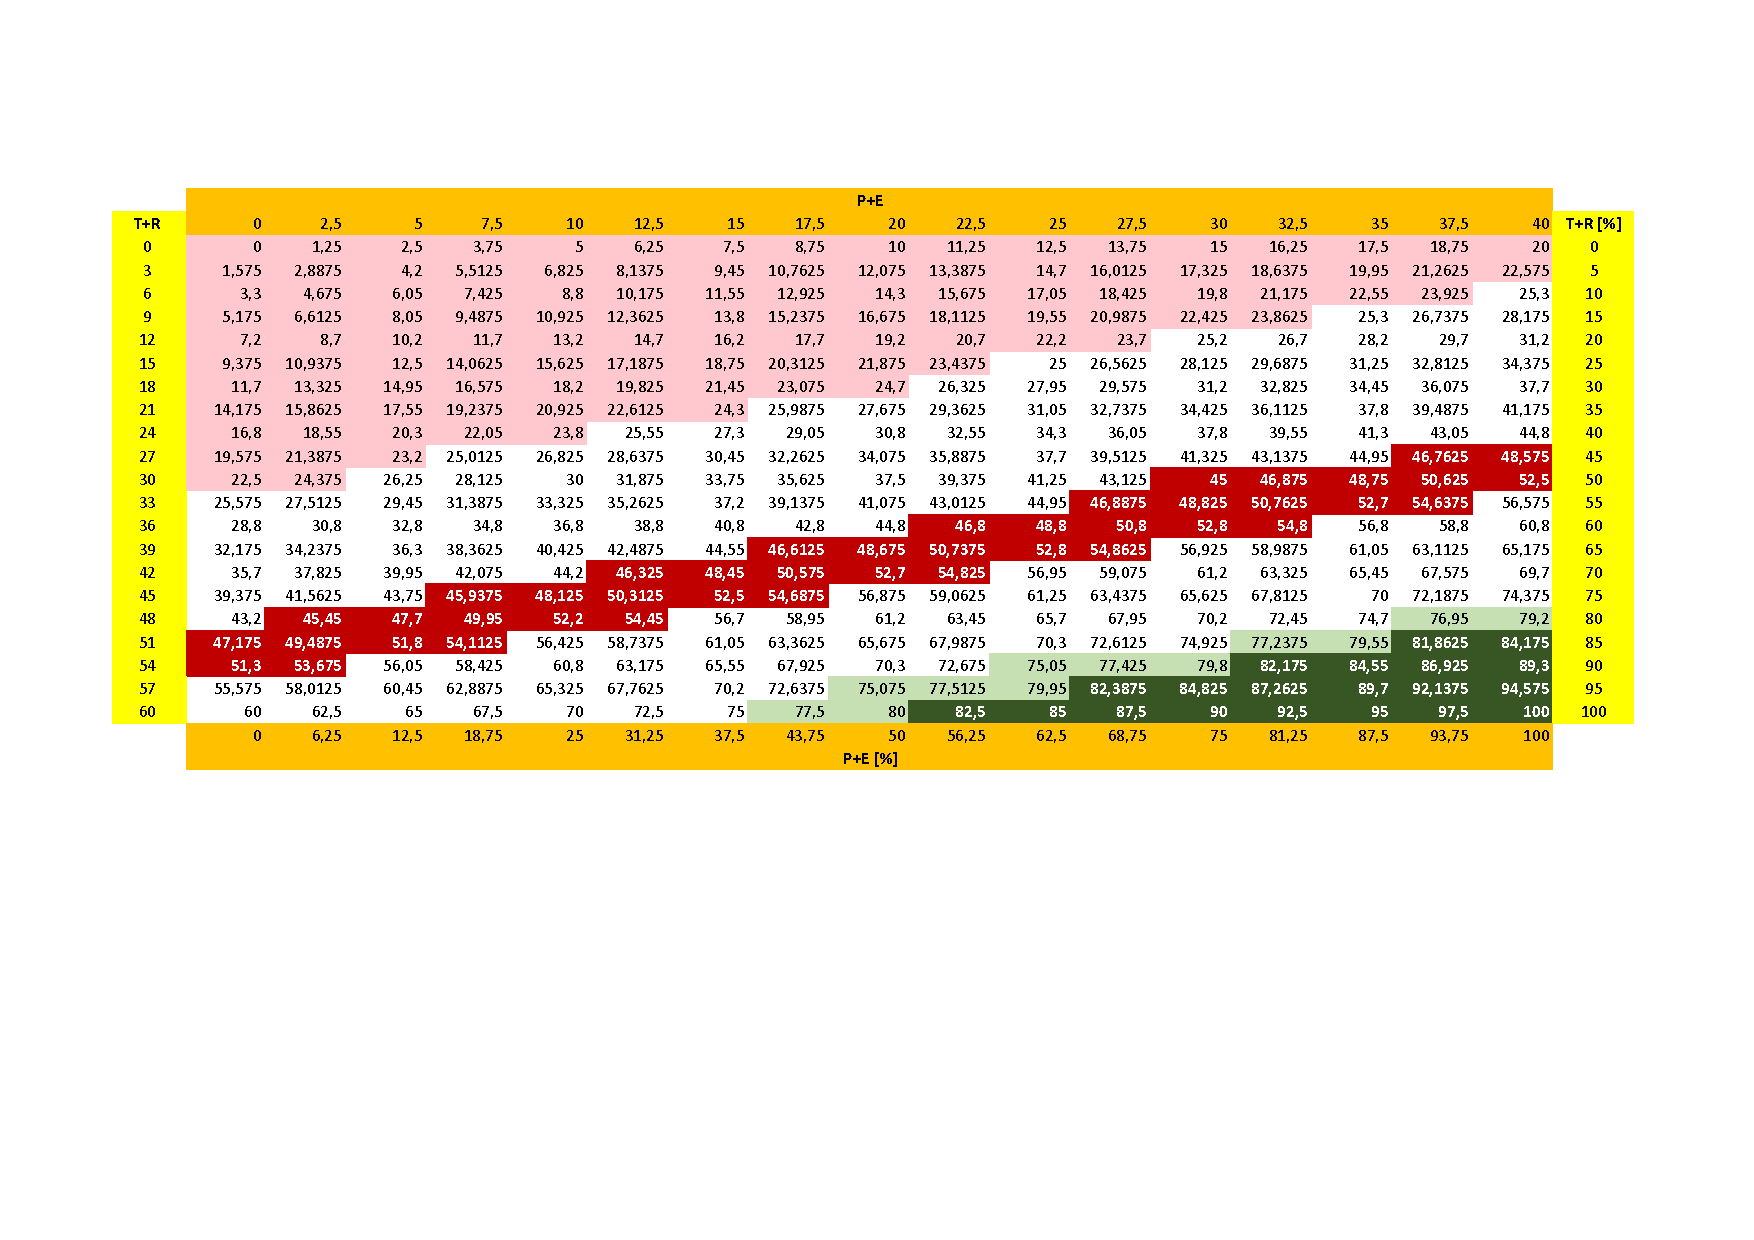
\includegraphics{eval-tbl.pdf}
}
\caption{Rozložení hodnocení dle $P$, $E$, $T$, $R$ pro (výchozí hodnoty) $K_1=K_2=0.5$}
\label{tbl:eval}
\end{table}


\thispagestyle{fancy}


\chapter{Poznámky k prezentacím}

\label{chapt:prez}

\thispagestyle{fancy}

\vspace{-8mm}
Více viz např. \href{https://www.herout.net/tao-diplomky/}{Tao diplomky}, sekce ``Státnice'',
\href{https://www.em.muni.cz/student/5046-8-rad-jak-spravne-prezentovat}{8 rad z Muni}
aj.

\section{Obecná doporučení}

\raggedbottom

\subsection*{Čeho se držet?}

\begin{itemize}
\item[\faCheck]
Dbejte na \textbf{jasnou myšlenkovou linii} -- prezentace by měla směřovat ``odněkud někam'' a 
každé sdělení posluchačům by mělo jasně souviset s touto linií,
\item[\faCheck]
\textbf{mějte jasno} v zavedených symbolech, pojmech, názvosloví atp. a \textbf{používejte je správně} -- jen tak 
přesvědčíte posluchače, že se v dané problematice velmi dobře orientujete a ``víte, o čem mluvíte'',
\item[\faCheck]
buďte \textbf{srozumitelní}, \textbf{konzistentní/bezesporní} a svá \textbf{tvrzení dokládejte} (daty, jejich zdrojem atp.),
\item[\faCheck]
\textbf{buďte konkrétní} -- vše se obvykle nějak jmenuje, přístupy jsou publikovány, množství, velikost či díl jdou vyjádřit číslem\footnote{(ideálně kvalifikovaný či řádový) číselný odhad je lepší než psát ``několik'', ``rychle'', ``okamžitě'' apod.} atp.
\item[\faCheck]
\textbf{text} na prezentačních snímcích \textbf{uvádějte} co nejvíce \textbf{kontrastně} a \textbf{heslovitě}, rozviňte jej až slovně; případné 
ilustrace používejte k objasnění, grafické efekty používejte velmi zřídka.
\end{itemize}

\subsection*{Čemu se vyhnout?\footnote{pro ilustraci viz např. \url{https://youtu.be/EzfZuVsIQMk}}}

\begin{itemize}
\item[\faClose]
\textbf{Čtení} textu prezentace ``\textbf{slovo od slova}'',
\item[\faClose]
\textbf{mluvení o nepodstatném}, 
\textbf{neudržování očního kontaktu} s posluchači\footnote{nadměrné pozorování špiček bot či poznámek, upření pohledu na strop/stěnu atp.}
či dokonce
\textbf{zády} k publiku,
\item[\faClose]
\textbf{používání a opakování} ``vycpávkových''\footnote{např. ``vlastně'', ``(tak)že'', ``jako'', ``prostě''} či 
jinak nevhodných\footnote{např. ``fíčura'', z angl. ``feature'' místo českého ``vlastnost/rys'' či ``pík'', z angl. ``peak'' místo česk. ``vrchol''} slov 
slovních spojení apod.,
\item[\faClose]
\textbf{rušení prezentace} zvoněním vlastního telefonu atp.
\end{itemize}


\section{Jak na prezentaci?}
\begin{enumerate}
\item
Abyste mohli vytvořit kvalitní prezentaci, \textbf{ujasněte si} nejprve:

\qquad

\tikzstyle{background rectangle}=[thin,draw=black]

\begin{savenotes}
\begin{tikzpicture}[show background rectangle, rounded corners=5pt]

\node[align=justify, text width=0.9\textwidth, inner sep=.5em]{
\vspace{-2mm}
\begin{itemize}
\item
\textbf{co} chcete sdělit (prezentovat),
\item
\textbf{komu} je sdělení určeno\footnote{tj., jaké posluchače předpokládáte -- kolegové z oboru, hodnoticí komise, zákazníci, veřejnost atp.} 
a 
jaký je jeho \textbf{účel}\footnote{tj., co od něj posluchači očekávají -- povzbuzení, rozbor problematiky, detaily k řešení, jeho obhajobu atp.}
\item
\textbf{kolik času}\footnote{dle něj stanovíte např. vhodný počet snímků prezentace, průměrný čas na jeden snímek apod.} na sdělení \textbf{máte},
\item
\textbf{v jakém prostředí} budete prezentovat\footnote{např. velikost prezentační plochy a její vzdálenost od posluchačů, světelné podmínky, možnost přehrát zvuk, video či přistoupit na internet}.
\end{itemize}
};

\node[xshift=3ex, yshift=0ex, overlay, fill=white, draw=white, above 
right] at (current bounding box.north west) {
\parbox{3mm}{\rotatebox{0}{\scalebox{1.5}{\faThumbTack}}\vspace{-2mm}}
};

\end{tikzpicture} 
\end{savenotes}


\item \textbf{Připravte si} sdělení, několikrát si je zkuste ``nanečisto'' a následně je \textbf{prezentujte}\footnote{díky nervozitě, neobvyklosti situace apod. může ``ostrá'' prezentace trvat (více či méně) déle}; 
každé srozumitelné sdělení má, obecně, \textbf{tři části}: 

\begin{description}
  \item [Začátek] (do $10$ \% času vyhrazeného pro prezentaci) ~ 

\begin{enumerate}
\item Nejprve \textbf{stručně představte}

 
\begin{itemize}
\item
\textbf{sebe}\footnote{stačí velmi stručně, např. jméno a příjmení}, 
\item
\textbf{účel/důvod}\footnote{stačí velmi stručně, např. obhajoba řešení \ldots} prezentace, 
\item
\textbf{téma}\footnote{obvykle název projektu}, které chcete posluchačům přiblížit, 
\item
případného \textbf{vedoucího}, popř. tým, pod kterým bylo téma řešeno,
\item
očekávaný \textbf{výsledek}\footnote{algoritmus/metoda, software, hardware či jejich kombinace, které jeho části považujete za stěžejní atp.} řešení tématu.
\end{itemize}

\quad 

\tikzstyle{background rectangle}=[thin,draw=black]

\begin{savenotes}
\hspace{2mm}
\begin{tikzpicture}[show background rectangle, rounded corners=5pt]

\node[align=justify, text width=0.75\textwidth, inner sep=.5em]{
\vspace{-2mm}
Tato část sice, zpravidla, \textbf{trvá cca 30 sekund}, ale \textbf{první dojem je} velmi \textbf{důležitý}!
};

\node[xshift=3ex, yshift=0ex, overlay, fill=white, draw=white, above 
right] at (current bounding box.north west) {
\parbox{3mm}{\rotatebox{0}{\scalebox{1.5}{\faThumbTack}}\vspace{-2mm}}
};

\end{tikzpicture} 
\end{savenotes}

\vspace{1mm}


\item 
\textbf{Následně} představte\footnote{spíše přehledově a do šířky než vyčerpávajícím způsobem a do hloubky}
\begin{itemize}
\item
\textbf{problematiku} související s daným tématem\footnote{``Co je na ní obtížné/zajímavé ?'', 
``Pomocí čeho (prostředky) a jak (metody) ji řešili jiní a s jakými výsledky?''
} -- ``jeden obrázek je více než sto slov'',
\item
\textbf{motivaci}\footnote{zabývat se daným tématem, když se jím zabývali jiní (nedostatky předchozích přístupů, námět na inovaci, přibyl aktuální problém atp.), tj. ``Proč/jaký má smysl zabývat se něčím obdobným?'', ``Čeho chcete dosáhnout?''} 
a \textbf{přínos}\footnote{(nového) řešení dané problematiky, tj. ``Co chcete vyřešit/zlepšit?''}
-- buďte co nejvíce konkrétní, podpořte svá tvrzení daty atp.,
\end{itemize}

\end{enumerate}

  \item [Střed] (cca $60$ \% času vyhrazeného pro prezentaci) ~

\begin{enumerate}
\item[]
\ldots představte
\begin{itemize}
\item
\textbf{Zvažované přístupy} k vlastnímu řešení vč. konkrétních \textbf{prostředků}, \textbf{technologií}, \textbf{metod}, jejich ne/výhod
a z jejich rozboru plynoucí \textbf{zvolený přístup}\footnote{přehledově, blokově, klíčové prvky a jejich vazby, mechanismus činnosti, případy užití apod.},
\item
\textbf{harmonogram} realizačních činností\footnote{zdůrazněte ty, které považujete za stěžejní, nejvíce náročné}, 
\item
\textbf{prvotní} řešení a, byť jen dílčí, \textbf{výsledky}\footnote{dosažené pomocí simulátoru, prototypu apod.} částečně/zcela potvrzující či vyvracející stanovená očekávání a odůvodňující/podporující zvolený směr řešení, 
\item
očekávané/zjištěné \textbf{překážky} v řešení, přístup k \textbf{jejich překonání}
a
\textbf{konečné} řešení.
\end{itemize}
\end{enumerate}

  \item [Konec] (cca $30$ \% času vyhrazeného pro prezentaci) ~

\begin{enumerate}
\item[]
\ldots představte
\begin{itemize}
\item
Zvolený přístup\footnote{podmínky/scénáře, datové sady, prostředky a metody sběru, zpracování a vizualizace dat atp.} k  \textbf{zhodnocení řešení}, 
\item
(vybrané) \textbf{stěžejní výsledky},
\item
vhodnými \textbf{daty podpořený}, jasný a kriticky pojatý \textbf{závěr}, tj. ``Co se ne/povedlo?''\footnote{jaké má řešené vlastnosti na jaké třídě aplikací, za jakých podmínek atp.},
\item
snímek\footnote{např. ``Děkuji za pozornost'', vhodná ilustrace apod.}, ze kterého prezentující i publikum jasně poznají, že prezentace skončila.
\end{itemize}
\end{enumerate}
  
\end{description}

\end{enumerate}

\raggedbottom

\quad


\chapter{Různé}


\thispagestyle{fancy}

\vspace{-8mm}

\section{Sazba s přijatelným množstvím ``bílého místa''}
\label{sec:C-1}

\vspace{-2mm}


\begin{figure}[h]
  \begin{floatrow}
     \ffigbox[2.0\FBwidth]
    {
\scalebox{5.0}{
	\faLineChart
}
    }
    {\caption{Ilustrace k \ldots}
    \label{fig:C-1}
  }
  \capbtabbox[2.0\FBwidth]{
\scalebox{5.0}{
	\faTable
}
     }{
      \caption{Data k \ldots}
      \label{tbl:C-1}
  }
  \end{floatrow}
\end{figure}


\section{Sazba se zbytečně velkým množstvím ``bílého místa''}
\label{sec:C-2}
\vspace{-2mm}

\begin{figure}[h]
\centering
\scalebox{5.0}{
	\faLineChart
}
\caption{Ilustrace k \ldots}
\label{fig:C-2}
\end{figure}

\begin{table}[h]
\centering
\scalebox{5.0}{
	\faTable
}
\caption{Data k \ldots}
\label{tbl:C-2}
\end{table}

\section{Výčet použitých doplňků}

(existují ale mnohé další a možná i lepší \ldots)

\begin{description}
\item[Balíky] (angl. packages)
\texttt{datetime2}, \texttt{floatrow}, \texttt{fontawesome}, \texttt{footnote}, \texttt{geometry}, \texttt{pdftex}, \texttt{tikz} (+ lib. \texttt{backgrounds}, \texttt{mindmap}), \texttt{tocloft}
\end{description}

\section{Výběr užitečných std. příkazů, prostředí atd. z \LaTeX}

\begin{description}
\item[Příkazy] 
\verb|\chapter|,
\verb|\section|,
\verb|\section*|,
\verb|\subsection|,
\verb|\subsection*|,
%
\verb|\label|,
\verb|\ref|,
\verb|\pageref|,
%
\verb|\pagestyle|,
\verb|\pagebreak|,
\verb|\newpage|,
\verb|\newline|,
\verb|\newcommand|,
\verb|\renewcommand|,
%
\verb|\centering|,
\verb|\flushleft|,
\verb|\flushright|,
\verb|\linewidth|,
\verb|\vspace|,
\verb|\hspace|,
\verb|\vfill|,
\verb|\smallskip|,
\verb|\medskip|,
\verb|\bigskip|,
\verb|\quad|,
\verb|\qquad|,
%
\verb|\parbox|,
\verb|\scalebox|,
\verb|\fbox|,
\verb|\colorbox|,
\verb|\includegraphics|,
%
\verb|\emph|,
\verb|\textbf|,
\verb|\textsc|,
\verb|\texttt|,
\verb|\footnote|,
%
\verb|\Huge|,
\verb|\huge|,
\verb|\LARGE|,
\verb|\Large|,
\verb|\large|,
\verb|\normalsize|,
\verb|\small|,
\verb|\footnotesize|,
\verb|\scriptsize|,
\verb|\tiny|,
%
\verb|\dots|,
\verb|\cdots|,
\verb|\ldots|,
\verb|\hyphenation|,
\verb|\overline|,
\verb|\underline|,
\verb|\overbrace|,
\verb|\underbrace|, 
\dots
\end{description}



\begin{description}
\item[Prostředí] 
\verb|\begin{name}| \ldots \verb|\end{name}|,
kde
\verb|name| =  
\verb|description|,
\verb|document|,
\verb|itemize|,
\verb|enumerate|,
\verb|figure|,
\verb|figure*|,
\verb|tabular|,
\verb|table|,
\verb|table*|,
\verb|equation|,
\verb|equation*|,
\dots
\end{description}


\label{lastpage}

\end{document}
